\documentclass[10pt,a4paper]{article}
%%%%%%%%%%%%%%%%%%%%%%%%%%%
% MODIFY:

\newcommand{\authorA}{Ahmad Bin Qasim (03693345)}
\newcommand{\authorB}{Kaan Atukalp (03709123)}
\newcommand{\authorC}{Martin Meinel (03710370)}
\newcommand{\groupNumber}{H} % - YOUR GROUP NUMBER
\newcommand{\exerciseNumber}{6} % - THE NUMBER OF THE EXERCISE
\newcommand{\sourceCodeLink}{https://gitlab.lrz.de/ga53rog/praktikum-ml-crowd}

\newcommand{\workPerAuthor}{
\authorA&Task 1&33\%\\
      &Task 2&33\%\\
      &Task 3&33\%\\
      &Task 4&33\%\\
    
      \hline
\authorB&Task 1&33\%\\
      &Task 2&33\%\\
      &Task 3&33\%\\
      &Task 4&33\%\\
    
      \hline
\authorC&Task 1&33\%\\
      &Task 2&33\%\\
      &Task 3&33\%\\
      &Task 4&33\%\\
   
}

%%%%%%%%%%%%%%%%%%%%%%%%%%%

%%
% imports for the exercise sheets
%

\usepackage[utf8]{inputenc}
\usepackage{amsmath}
\usepackage{amsfonts}
\usepackage{amssymb}

\usepackage[yyyymmdd]{datetime}
\renewcommand{\dateseparator}{--}

\usepackage[left=2cm,right=2cm,top=3cm,bottom=3cm]{geometry}

\usepackage{hyperref}

\usepackage{amsthm}
\newtheorem{lem}{Lemma}
\newtheorem{thm}{Theorem}
\newtheorem{cor}{Corollary}
\newtheorem{rem}{Remark}
\newtheorem{definition}{Definition}
\newtheorem{ter}{Terminology}

\usepackage{graphicx}

\newcommand{\M}{\mathcal{M}}
\newcommand{\N}{\mathcal{N}}
\newcommand{\K}{\mathcal{K}}
\newcommand{\SPDk}{\mathbb{P}^k}
\newcommand{\vol}{\text{vol}}

\newcommand{\Figref}[1]{Figure~\ref{#1}}
\newcommand{\figref}[1]{figure~\ref{#1}}
\newcommand{\Eqnref}[1]{Equation~(\eqref{#1})}
\newcommand{\eqnref}[1]{equation~(\eqref{#1})}

\usepackage{float}
\usepackage{tabularx}
\usepackage{subcaption}
\usepackage{mwe}

\usepackage{fancyhdr}
\pagestyle{fancy}

\usepackage{totcount}
\newtotcounter{taskCounter}
\newtotcounter{pointCounter}
\newenvironment{task}[1]{\noindent\stepcounter{taskCounter}\textbf{Report on task #1}\smallbreak\hrule\smallbreak}{\smallbreak\hrule\bigbreak}


\title{Report for exercise \exerciseNumber~from group~\groupNumber}

\makeatletter
\let\thetitle\@title
\let\theauthor\@author
\let\thedate\@date
\makeatother

\providecommand{\versiondate}{\today}

\lhead{Exercise sheet \exerciseNumber}
\chead{Master Praktikum: Modelling and Simulation of Crowds WS2019/20}
\rhead{TUM}
\lfoot{Report of Group \groupNumber}
\cfoot{\thepage}
\rfoot{Last compiled: \versiondate}
\renewcommand{\headrulewidth}{0.4pt}
\renewcommand{\footrulewidth}{0.4pt}

\newcommand{\frontpage}{
\begin{center}
\textbf{\thetitle}\\~\\
\end{center}
\begin{table}[H]
\begin{tabular}{ll}
Tasks addressed:&\total{taskCounter}\\
Authors:&\authorA\\
&\authorB\\
&\authorC\\
Last compiled:&\versiondate\\
Source code:&\sourceCodeLink
\end{tabular}
\end{table}
\vfill
The work on tasks was divided in the following way:
\begin{table}[H]
\begin{tabularx}{\textwidth}{X|p{2cm}|p{2cm}}
\workPerAuthor
\end{tabularx}
\end{table}
\newpage
}

\begin{document}

\frontpage

\begin{task}{1, Performing a literature review on the topic of trajectory prediction}
    \textbf{Problem statement of trajectory prediction.} \bigbreak
    The problem of understanding and forecasting the trajectory of humans is becoming more important during the recent years, with the rise of autonomous systems. Forecasting trajectories plays a central role in the fields of autonomous driving, service robots or smart surveillance systems. \\
    Human behavior is difficult to predict for an algorithm because it can be influenced by a multitude of hidden factors. Human motion behavior is not an exception, it can be influenced by the intent of a person, the people surrounding a person, social rules of the environment and even the personality traits of the person. Due to this, motion behavior forecasting is a challenging problem. \\
    Human motion behavior can constitute a diverse set of behaviors such as gestures, facial expressions, movement of limbs etc. but for this project our aim was the forecasting of human movement in 2D space. \\
    Movement in 2D space forecasting can be classified into two types, human-space interactions and human-human interactions forecasting. The former, predicts the interactions between humans and the environment such as obstacle avoidance while the latter aim to forecast the interactions among human subjects. Specifically, this project focuses on human-human interactions. \\
    When it comes to human-human interactions, the following are the properties of human motion:
    
    \begin{itemize}
        \item Interpersonal aspects: People surrounding a person, some trajectories are not physically possible because of the presence of other people around a subject.
        \item Social aspects: Some trajectories are physically possible but they are not socially acceptable.
        \item Multimodal: There can be multiple good trajectories that a person can take.
    \end{itemize}
    
    \bigbreak
    
    \begin{figure}[H]
    \centering
    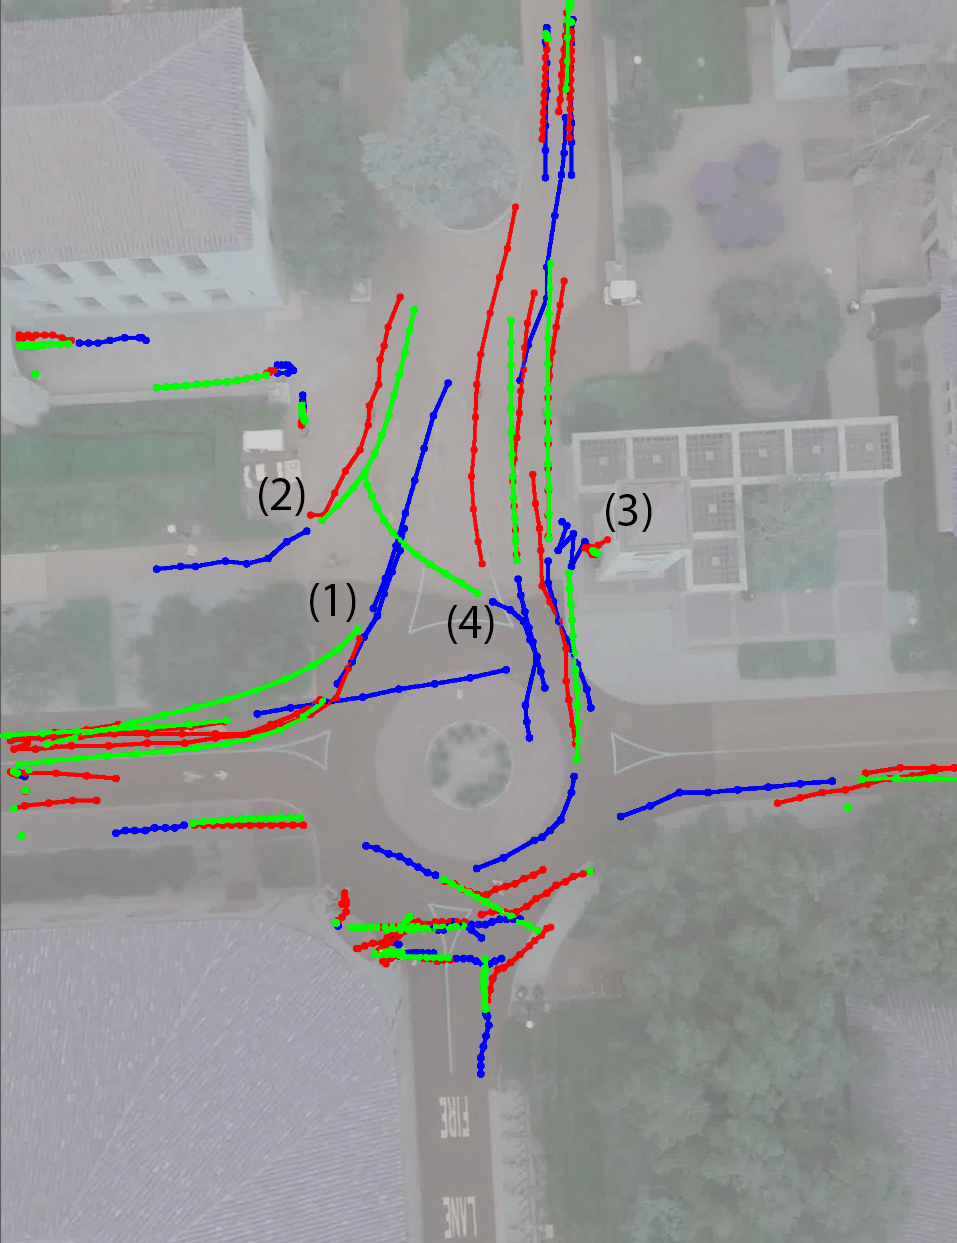
\includegraphics[scale=0.175]{pictures/example_trajectory.png}
    \caption{A screenshot from the stanford drone dataset, which highlights the complexity of human motion behavior. The colored lines show the trajectory taken by different pedestrians in an urban environment}
    \label{fig:example_trajectory}
    \end{figure}
    
    There are three approaches in the research literature which are used for finding a solution for the problem of trajectory prediction which are given here:
    
    \begin{itemize}
        \item Hand-crafted models: Models which use fixed rules and hand-crafted energy potentials \cite{laura}
        \item Recurrent Neural Nerwork (RNN) based models: Models which try to harness the time-series data prediction capabilities of RNNs.
        \item Generative models: Generative models like Variational Autoencoders \cite{vae} aim to model the distribution of the training data. Generative Adversarial Networks (GANs) \cite{gan}, are a relatively newer addition.
    \end{itemize}
    
    \newpage
    
    Now we will provide an overview of the three approaches mentioned before. We will review an example that we found interesting for each of the approach and summarize it in a few paragraphs. \bigbreak
    
    \textbf{As an example for hand-crafted models we reviewed: "Learning an image-based motion context for multiple people tracking" \cite{laura}} \\
    
    \textbf{Motivation}\\
    In computer vision you often want to detect and track multiple people since they are often the center of attention of a scene. This problem is often tackled by estimating the location of each pedestrian by using a detector for each frame. These locations are associated in time to build consistent tracks for each individual. \\ This approach has the disadvantage of highly depending on the detection results. In semi-crowded environments it often occurs that individuals are hidden and cannot be detected properly. This is why it is very hard to estimate a pedestrian's trajectory.\\
    This paper constructs a model approximating the movement of a pedestrian according to motion and appearance features in his environment. So it relaxes the dependency on detections. One application field is the pedestrian intention detection which is important for autonomous car navigation.\\
    \textbf{Method}\\
    The method is based on so called "interaction feature strings" encoding image features of a particular scene. A scene is defined as an area centered around a detected pedestrian i at a certain time t and a position (x,y). Each scene is divided into several blocks and a set of features is computed for each block. The interaction feature string is the concatenation of the block features over all blocks of a scene. The features which are used include Mean Optical Flow (MOF), Difference Optical Flow (DOF), Histogram of Optical Flows (HOF), Ternary Optical Flow (TOF), Ternary Angular Optical Flow (TAOF). 
    After having a descriptive set of features for a scene a  Random Forest is trained to estimate the velocity of a pedestrian. \\
    More in detail the method computes the interaction feature string from low-level features for a scene. This is given as input for the Random Forest which outputs the most likely pedestrian velocity. This is then given as an input to a probabilistic tracking framework (e.g Linear Programming) to get the final set of trajectories.\\
    The random forest consists of random trees which are trained on mapping a feature string to the velocity of a pedestrian.\\
    \textbf{Results}\\
    The performance of the method was compared against the Social Force Model and the Optical Flow in estimating the velocity of a pedestrian. Figure \ref{fig:degree_error} shows the error in degrees of each method in a). So it can be easily seen that the new method is able to estimate it up to 20 degrees more accurately in comparison to SFM and up to 40 degrees more accurately compared to Optical Flow. Furthermore b), c) and d) show the histogram of velocity estimation errors given by the different methods. From there you can read that the new method makes more than 50\% of the estimation with less than 10 degrees of errors, while Optical Flow Model and Social Force Model can only produce 20\% and 30\% of their estimations with these low amount of errors.
    \begin{figure}[H]
        \centering
        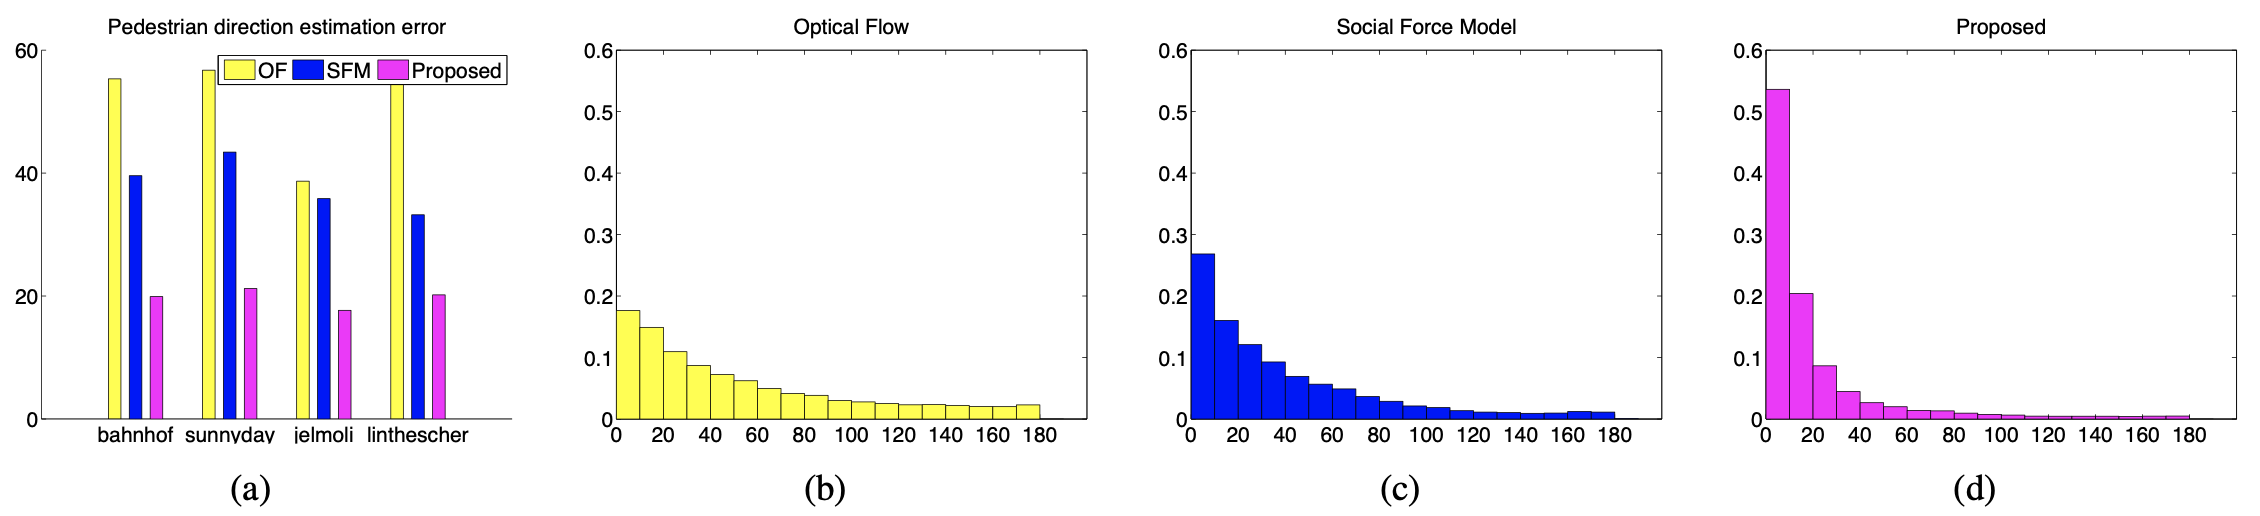
\includegraphics[width=\textwidth]{pictures/errors.png}
        \caption{Estimated error in degrees of pedestrian velocity using Optical Flow, SFM and the proposed method \cite{laura}}
    \label{fig:degree_error}
    \end{figure}
    Figure \ref{fig:examples} shows pictures with the estimated velocity of the model in red and the ground truth velocity in green. It can be seen that the accuracy is high.
    \begin{figure}[H]
        \centering
        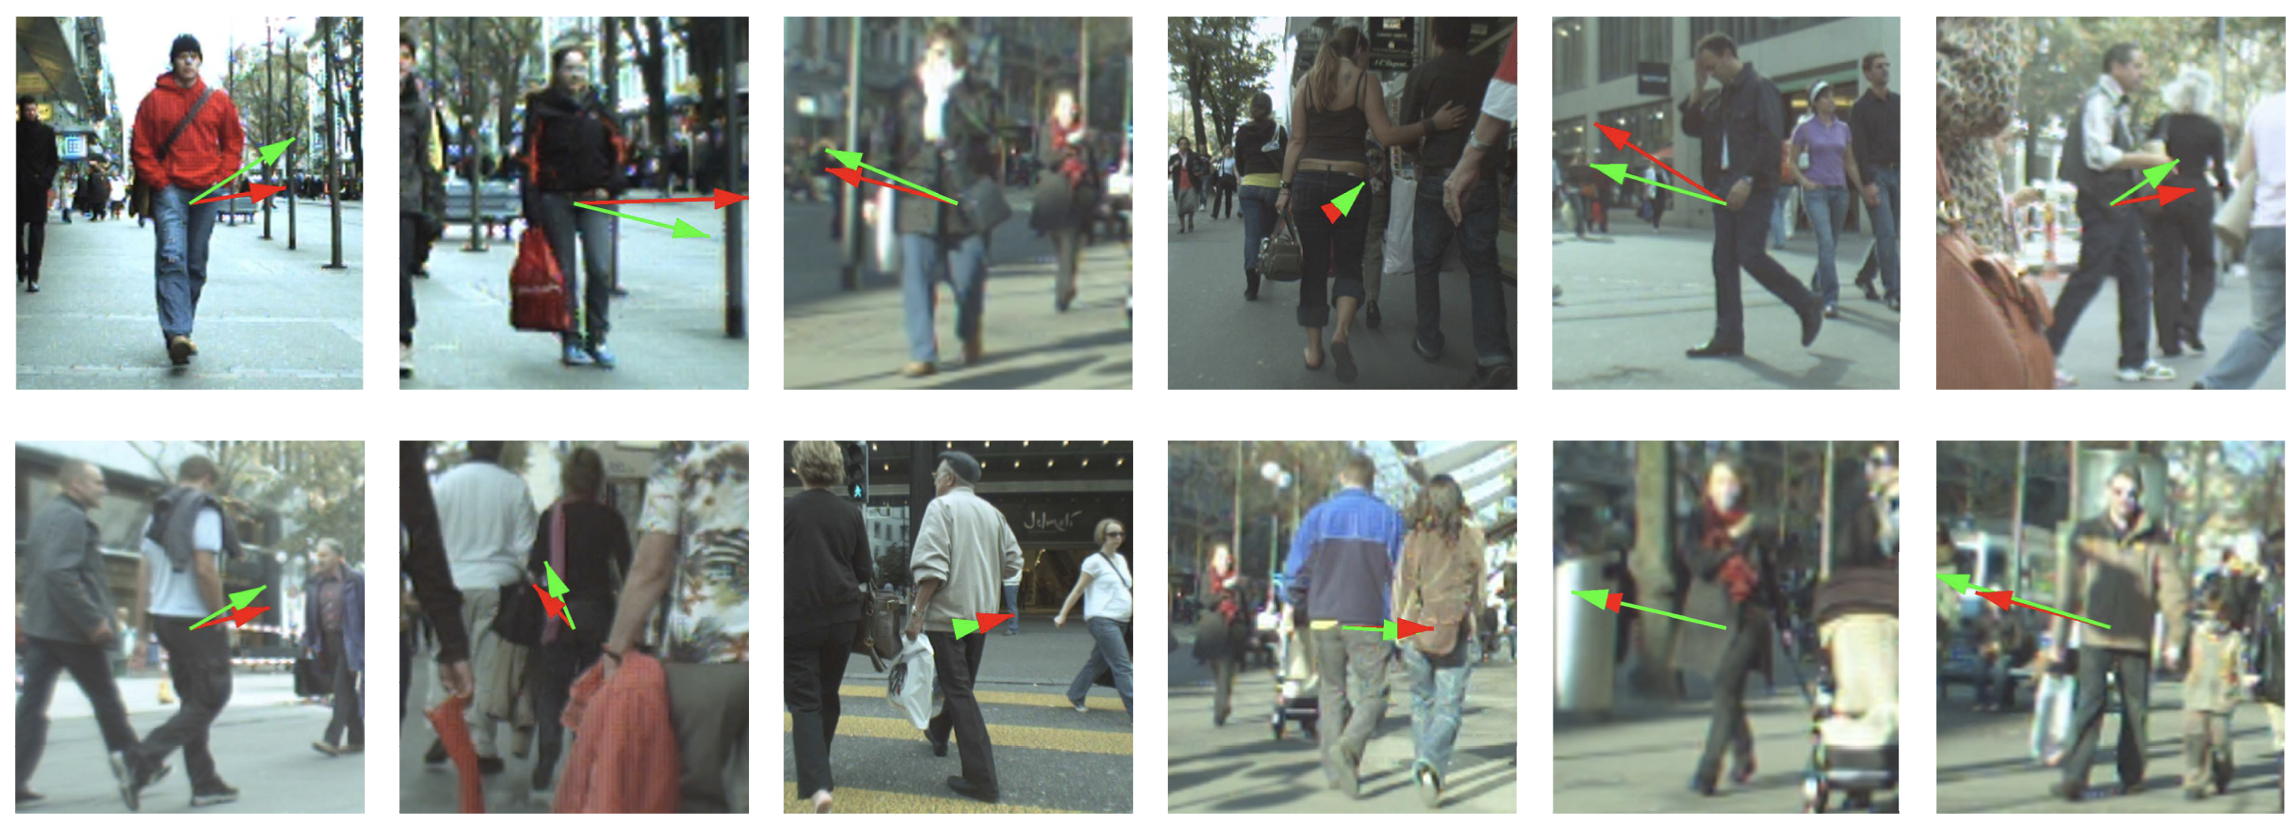
\includegraphics[width=\textwidth]{pictures/examples.png}
        \caption{Examples of pedestrian's estimated velocity. The ground truth is marked in green, while the model estimation is marked in red \cite{laura}}
        \label{fig:examples}
    \end{figure}

    \textbf{As an example of RNN-based models we reviewed: "Social LSTM: Human Trajectory Prediction in Crowded Spaces" \cite{social_pooling}} \\
    
    \textbf{Motivation} \\
    The aim of the paper is to predict human-human interactions in the domain of human motion behavior. The authors try to especially model the social aspects of human motion. They do this by introducing a Social Pooling (SP), layer which allows the LSTM to share their hidden states.
    
    \textbf{Method}
    The input to the model are x and y coordinates of the pedestrians in the scene. Authors use LSTMs \cite{lstm}, to learn the time series of coordinates of pedestrians positions in the scene. Specifically, within the model there is one LSTM per person in the scene. Using LSTMs, for each person's trajectory is a viable approach but in such an architecture each LSTM is agnostic of the hidden state of other LSTMs. Hence, the predicted trajectories from a single LSTM for a single pedestrians is not influenced by other pedestrians in the scene. In order to achieve the aim of modeling human-human interactions, the authors present a novel approach called social pooling. \ref{fig:social_lstm}
    
    \begin{figure}[H]
        \centering
        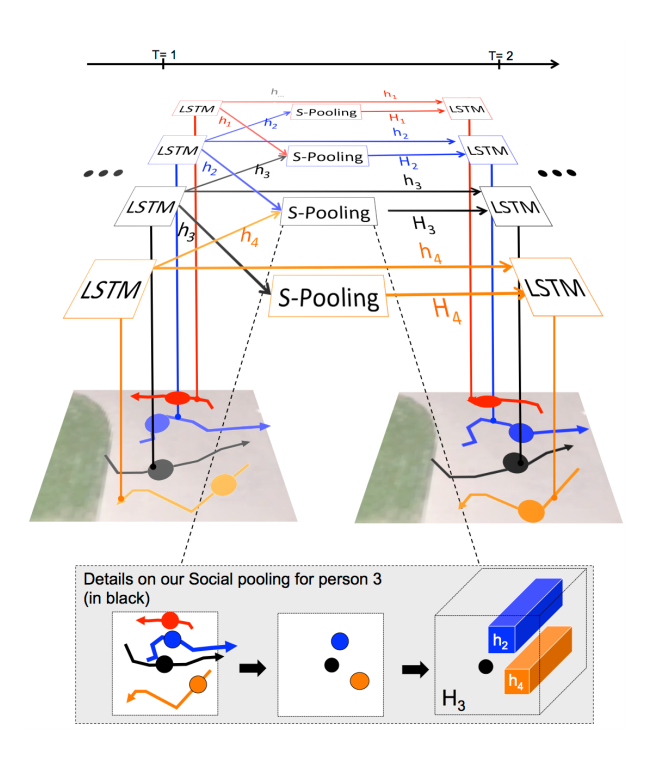
\includegraphics[scale=0.25]{pictures/SocialLSTM.png}
        \caption{The architecture of SocialLSTM shows, per-pedestrian LSTMs and the social pooling layer which combines the hidden state of neighboring pedestrian LSTMs}
        \label{fig:social_lstm}
    \end{figure}
    
    At every timestep, each LSTM (modeling the prediction of a single person), receives the socially pooled hidden state of neighboring LSTMs. These pooled hidden states contain all the information for the LSTM cell to make socially aware predictions.
    
    \textbf{Results}
    
    SocialLSTM has better results compared to the SocialGAN \cite{gupta2018social} paper that we have implemented during this project. Although we chose SocialGAN because predicting trajectories using it is less computationally expensive with a small compromise on the results (more about this in section 2 when we provide more details of SocialGAN).
    
    \begin{tabular}{|l|c|c|}
         \hline
         \textbf{Metric}&\textbf{Dataset}&SocialLSTM\\
         \hline
         ADE&ETH&0.50\\
         FDE&ETH&1.07\\
         \hline
    \end{tabular} \bigbreak
    
    \textbf{As an example of the Generative models we reviewed: "DESIRE: Distant Future Prediction in Dynamic Scenes with Interacting Agents" \cite{desire}} \\
    
    \textbf{Motivation}\\
    The aim is to create a scalable, accurate and diverse model that predicts mutliple interacting agents' behaviour in a dynamical stochastic environment.\\
    \textbf{Method}\\
    The RNN-based computationally efficient prediction framework DESIRE has 2 modules: Sample Generation Module and Ranking \& Refinement Module. The Sample Generation Module generates hypothetical future predictions using a GRU-based conditional variational autoencoder and feeds them to the Ranking \& Refinement Module. That module assigns rewards to each hypothetical future prediction and refines the predictions by adding a displacement vector to them. The displacement vector is predicted with an NN regressor with iterative feedback at each cycle allowing the model to consider past data.\\
    \textbf{Conclusion}\\
    The prediction errors of DESIRE were noticeably lower than the simple autoencoder implementations and other baseline models on the publicly available KITTI and Stanford Drone Datasets. \\
    \end{task}

\begin{task}{2, GANs and the architecture of Social GAN}
    \textbf{Details of GANs: \cite{gan}} \bigbreak
    GAN is an abbreviation for Generative Adversarial Network which is popular for generating pictures or texts for example from some random noise. In our case we try to predict pedestrian trajectories from having some first steps for each pedestrian's trajectory.\\
    In general GANs always consists of a generator and a discriminator which work against each other. The generator always tries to create something for example a picture, while the discriminator tries to identify if the given input picture is a real picture or just a generated picture from the generator. The generator's goal is that the discriminator identifies the created pictures as real ones, while the discriminator's goal is to detect which pictures are "real ones" and which ones are just created by the generator.
    \\ We use now some mathematics to be more clear about GANs. In general every neural network can be a generator. We say a neural network $G(z,\theta_1)$ is used to model the generator. It uses the input noise $z$ and the weights $\theta_1$ to map $z$ to the data space $x$ which is for example a picture. A second neural network $D(x,\theta_2)$ models the discriminator and determines a probability if x belongs to the real data set or was created by the generator.\\
    Consequently the discriminator is trained to maximize the probability of classifying real images as real while minimizing the probability of classifying fake images as part of the real data set. So the loss function should maximize $D(x)$ and minimize $D(G(z))$.\\
    The generator is trained to fool the discriminator, so the parameters are trained to maximize the probability that any generated picture is classified as part of the real data set. This is why the loss function of the generator maximizes $D(G(z))$.\\
    At some point the training will converge where the discriminator nor the generator cannot improve anymore (i.e. Nash equilibrium) and ideally the generator creates realistic data so that the discriminator is unable to detect whether some input belongs to the real data set or not. \cite{gan} \\
    As already mentioned above the generator and discriminator are trained to optimize opposite loss functions. This can be expressed with following formula: 
    \begin{equation*}
        \min_{G}\max_{D}V(D,G) = \mathbb{E}_{x~p_{data}(x)}[\log D(x)]+\mathbb{E}_{z~p_{z}(z)}[\log (1-D(G(z)))] \cite{gan}
    \end{equation*}
    
    \textbf{Introduction and architecture of SocialGAN \cite{gupta2018social}:} \bigbreak
    In this paragraph we introduce the SocialGAN (SGAN) model. The SGAN aims to forecast the human-human interactions motion behavior. It is a generative model based on Generative Adversarial Networks. The three main components of the SGAN are generator and the discriminator. The generator consists of an encoder, a pooling module and a decoder. The discriminator is composed of an encoder only. Figure \ref{fig:sgan_architecture} visualizes the described architecture.
    \begin{figure}[H]
        \centering
        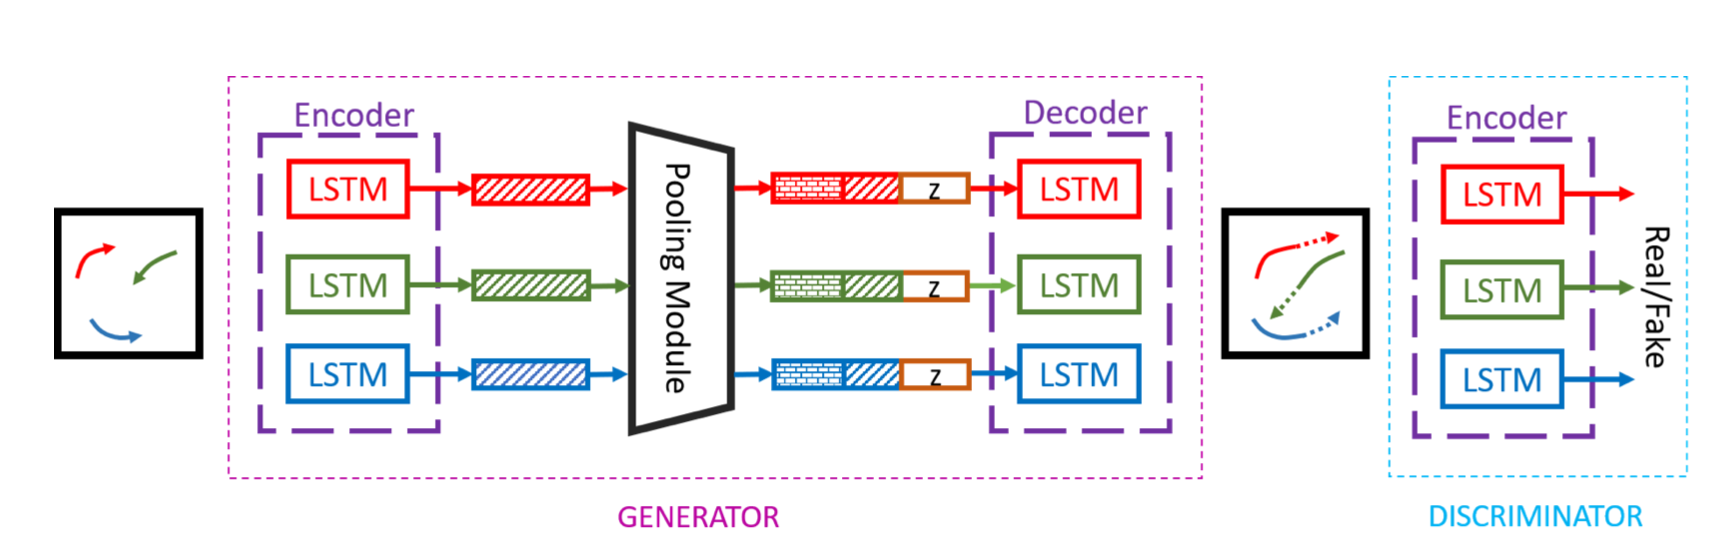
\includegraphics[width=0.7\textwidth]{pictures/SGAN_architecture.png}
        \caption{Architecture of the Social GAN \cite{gupta2018social}}
        \label{fig:sgan_architecture}
    \end{figure}
    The encoder network is comprised of an embedding layer and a one-layer LSTM \cite{lstm}. The encoder takes as input a time-series data and embeds it using a single linear layer. These embedded time-series coordinates are then passed through a LSTM. The encoder returns the hidden state as the encoded data. \\
    The input data of the generator is 3-dimensional and consists of trajectories of pedestrians with an x- and y-coordinate. The encoder is used in the generator for encoding the input data, as mentioned above, the encoder returns the hidden state of the one-layer LSTM in the encoder. The output is passed through a pooling module (PM). This is the novel addition that authors made.\\
    The PM is responsible for enforcing social behaviour of the pedestrians. Social Pooling (SP)\cite{social_pooling} is used by A. Alahi et. al. which serves the same purpose but it has a limitation i.e. due to social pooling the hidden layers of all the LSTMs are coupled together and at each time step, these coupled LSTMs have to be backpropagated which is a very computationally expensive step. The authors introduce PM which includes a multi-layer perceptron (MLP) with max pooling. PM allows different pedestrians to be considered together in a neural network, generally resulting in more "natural" trajectories such as walking in groups, avoiding crossovers, and following each other although the model becomes worse at correctly predicting the trajectories. \\
    As shown in Figure \ref{fig:pooling_module}, the pooling module takes the relative positions of the red person and all other persons and concatenates the embeddings of them with the hidden states of the LSTM from the encoder. These concatenations are then fed into a multi-layer perceptron and then processed through a maximum pooling layer.
    \begin{figure}[H]
        \centering
        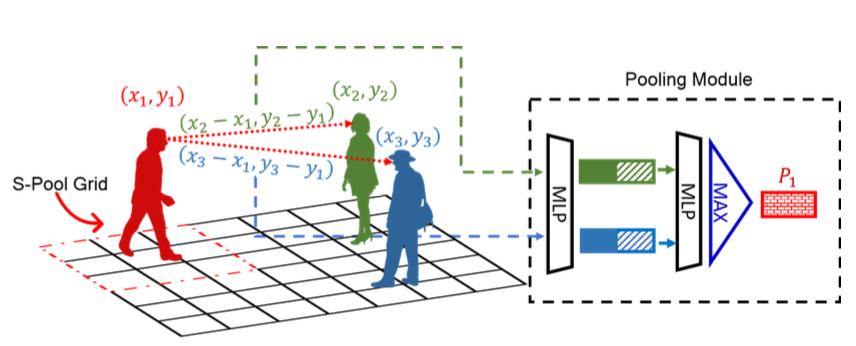
\includegraphics[width=0.7\textwidth]{pictures/pooling_module.png}
        \caption{Pooling module of the Social GAN \cite{gupta2018social}}
        \label{fig:pooling_module}
    \end{figure}
    The output of the pooling module is then concatenated with the output of the encoder and some additional noise and fed into the decoder. The decoder embeds the given input and forwards it into another one-layer LSTM. The output of this one-layer LSTM is then passed through a linear layer which transforms the input to a two-dimensional output, which corresponds to the predicted x- and y-coordinates for the next step. \bigbreak
    The input of the discriminator is similar to the data set of the generator but containing longer trajectories, because either the generated predictions or the ground truth predictions were concatenated.\\
    The discriminator encodes the input data using an encoder which has the same architecture as the encoder used within the generator. The purpose of the discriminator is to classify the given trajectories as "real" or "fake" data. This is why a MLP is applied on the encoded trajectories in order to obtain one classification score for each trajectory.\bigbreak
    Another novel component of the Social GAN paper is the variety loss, shown in equation \ref{eq:variety_loss}. This loss is used to encourage diverse samples. The problem of predicting trajectories is that there are often several trajectories which can be considered the accurate prediction, as mentioned in section 1. The method would just average the predictions in case of multiple possibilities. The variety loss encourages the network to compute k several possible trajectories for each scene and chooses the best prediction according to the $L_2$ loss. \cite{gupta2018social}
    \begin{equation}\label{eq:variety_loss}
        \mathcal{L}_{variety} = \min_k||Y_i - \hat{Y_i^{k}}||_2
    \end{equation}
\end{task}

\begin{task}{3, Implementation}
\begin{itemize}
    \item The encoder, decoder, discriminator, generator, and pooling module were implemented as separate classes. The discriminator has an encoder, and the generator has an encoder, a decoder, and a pooling module. During training the discriminator and generator objects are trained against each other. The generator is then used to generate samples during testing. \\ 
    \item The model was trained with 200 epochs and a batch size of 64. The encoder and decoder sizes were 16 and 32 respectively. Adam optimizer with a learning rate of 0.001 was used for training. A regularization term of 0.1 was used for the $L_2$ loss. Furthermore we used a value of 5 for the variational loss, because we were limited in size of the GPU. \\
    \item In the original implementation, the authors apply ReLU activation function to the output of the discriminator. These scores are then used to calculate the binary cross entropy (BCE) loss. As the bounds of the ReLU acivation function is between 0 and infinity, it doesn't make sense to use ReLU as the activation function. So we applied a sigmoid function before calculating the BCE loss.\\
    \item In our implementation we make use of the pooling module of the Social GAN paper.\\
    \item We used Microsoft's cloud computing service Azure to train our models. We picked a so called "Data Science Virtual Machine" containing necessary modules like PyTorch, virtual environments and CUDA support for faster training. 
\end{itemize}
\end{task}

\begin{task}{4, Results}

\begin{itemize}
    \item The data were collected from a camera set up at the entrance of a faculty building of ETH. The positions of the pedestrians leaving and entering the building were saved at each frame. The dataset contains the time frame, the id of the individual pedestrian, and his/her coordinates. \\
    \item Average Displacement Error (ADE) is the average of L2 distances of the predictions and the ground truth. Final Displacement Error (FDE) is the L2 distance of the final prediction point and the final real point. Both measures are in meters. \\
    \item Result comparison with the author's results.
    The following table shows the results from the Social GAN using the ADE and FDE metrics on the ETH data set.
    The first number of the model corresponds to the k of the variety loss. So for the first model it does not create different trajectories. For example, for the last model there are 20 trajectories predicted from which is taken the best one according to the $L_2$ loss. The second number corresponds to the number of samples, which are different predictions of the same observation. The ADE and FDE metrics are computed over all these predictions and the average is taken. The results of the paper's models and our results are as follows:\bigbreak
    \begin{table}[H]
        \centering
    \begin{tabular}{|l|c|c|c|c|c|c|c|}
    \hline
         \textbf{Metric}&\textbf{Dataset}&1V-1&1V-20&20V-20&20VP-20&5VP-20*&\textbf{5VP-20*}\\
         \hline
         ADE&ETH&0.79&0.75&0.61&0.60&0.61&0.46\\
         FDE&ETH&1.61&1.52&1.22&1.19&1.10&0.84\\
         \hline
    \end{tabular}
     \caption{Results of different models according to FDE and ADE metrics}
    \label{tab:results}
    \end{table}
    \bigbreak
   The first 4 models are the models trained by the authors of the SocialGAN paper. The last 2 ones are our trained models. The first starred one is trained with an observed trajectory length of 12 to predict the next 8 steps like the authors' models. The bold and starred one is trained with an observed trajectory length of 16, which explains the better performance.
   \item Table \ref{tab:results} shows comparable results for the 20V-20 and the 20VP-20 model, which are only different because the 20VP-20 model uses the pooling module but the other module does not. It can be seen that the performance is slightly the same. The authors even say that the SGAN without the pooling module achieves slightly better results than the SGAN using the pooling module. The reason why it is used even though is that it enforces social behaviour of the pedestrians.
   \item Some example predictions that we have found rather interesting are below:
\begin{figure}[H]
\centering
\begin{subfigure}[b]{0.475\textwidth}
\centering
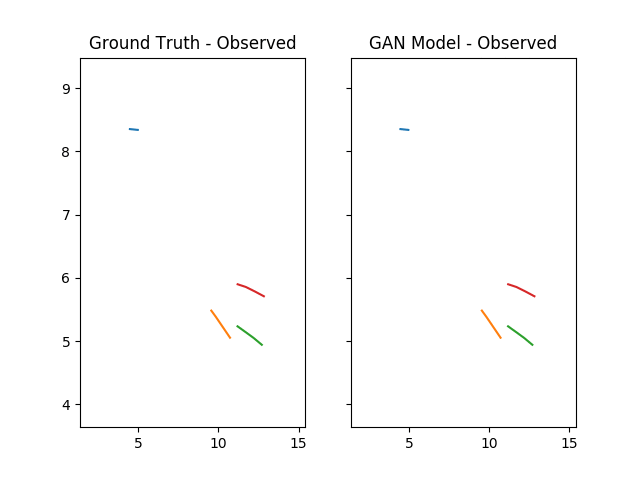
\includegraphics[width=\textwidth]{pictures/frames/follow/frame_03_delay-0,35s.png}
\caption[]
{{\small The initial position of all 3 pedestrians. The pedestrians are in orange, green and red colored lines.}}
\label{fig:follow_1}
\end{subfigure}
\hfill
\begin{subfigure}[b]{0.475\textwidth}
\centering
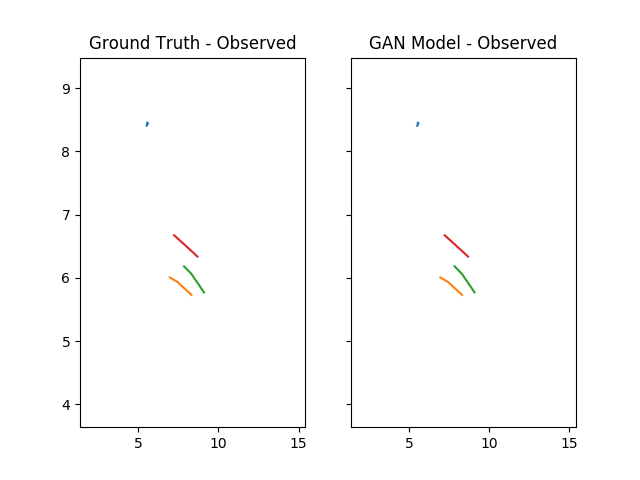
\includegraphics[width=\textwidth]{pictures/frames/follow/frame_11_delay-0,35s.png}
\caption[]
{{\small The orange and the green pedestrians, and the red pedestrian start to clash.}}
\label{fig:follow_2}
\end{subfigure}
\hfill
\vskip\baselineskip
\begin{subfigure}[b]{0.475\textwidth}
\centering
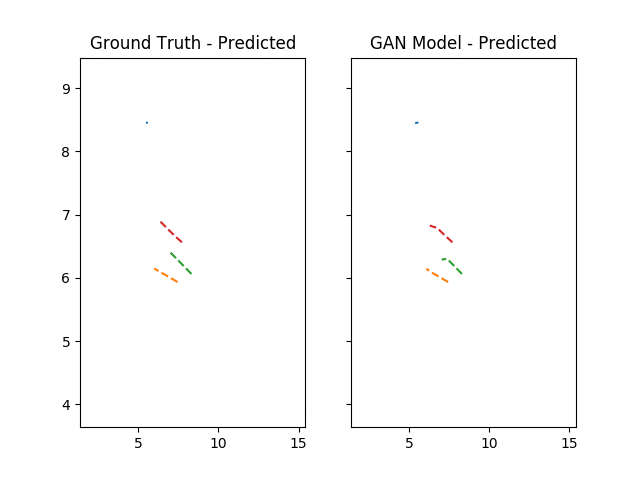
\includegraphics[width=\textwidth]{pictures/frames/follow/frame_13_delay-0,35s.png}
\caption[]
{{\small The green pedestrians starts to change its direction to the orange pedestrian in the prediction while, in ground truth its going straight}}
\label{fig:follow_3}
\end{subfigure}
\quad
\begin{subfigure}[b]{0.475\textwidth}
\centering
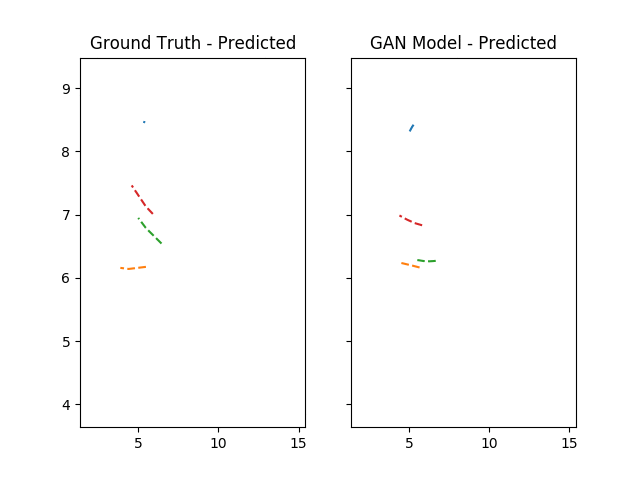
\includegraphics[width=\textwidth]{pictures/frames/follow/frame_17_delay-0,35s.png}
\caption[]
{{\small At the end, the green pedestrian follows the orange pedestrian, whereas at the ground truth it follows the red one}}
\label{fig:follow_4}
\end{subfigure}
\caption{Some observed and predicted frames of 3 pedestrians. The left graphs are the always the ground truth and the right graphs are the model's observed or predicted trajectories as seen in its title.}
\label{fig:follow}
\end{figure}



\begin{figure}[H]
\centering
\begin{subfigure}[b]{0.475\textwidth}
\centering
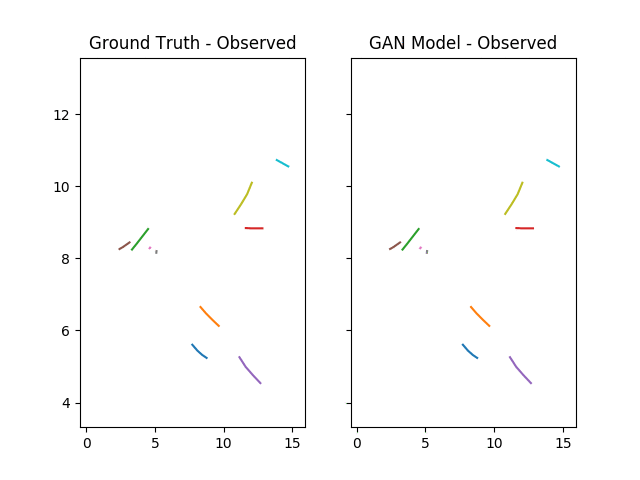
\includegraphics[width=\textwidth]{pictures/frames/chaotic/frame_01.png}
\caption[]
{{\small The initial position of all pedestrians.}}
\label{fig:chaotic_1}
\end{subfigure}
\hfill
\begin{subfigure}[b]{0.475\textwidth}
\centering
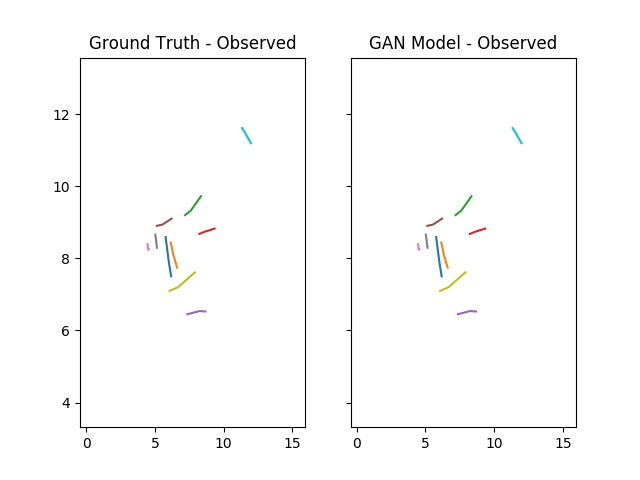
\includegraphics[width=\textwidth]{pictures/frames/chaotic/frame_10.png}
\caption[]
{{\small A clash of groups and individuals happens.}}
\label{fig:chaotic_2}
\end{subfigure}
\hfill
\vskip\baselineskip
\begin{subfigure}[b]{0.475\textwidth}
\centering
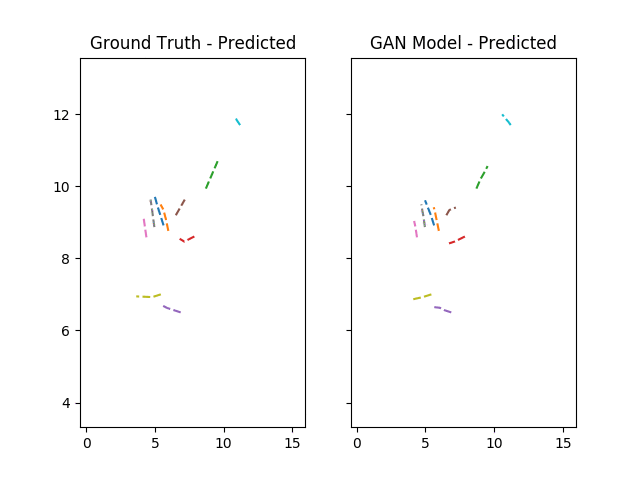
\includegraphics[width=\textwidth]{pictures/frames/chaotic/frame_14.png}
\caption[]
{{\small As soon as it starts predicting, our model assumes that the red pedestrians will not follow the group above him. The purple pedestrian starts to follow the yellow one.}}
\label{fig:chaotic_3}
\end{subfigure}
\quad
\begin{subfigure}[b]{0.475\textwidth}
\centering
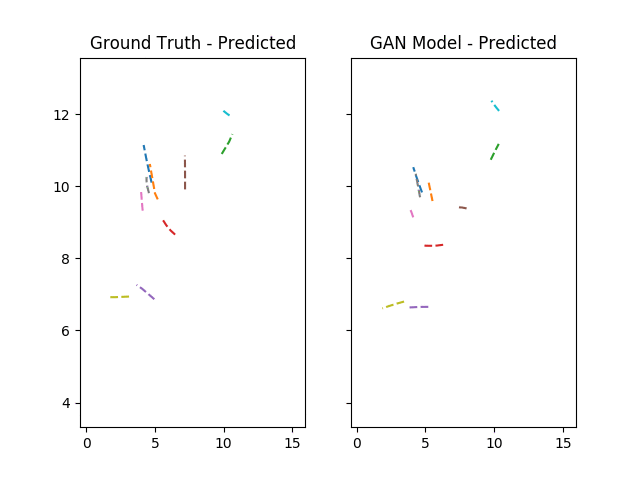
\includegraphics[width=\textwidth]{pictures/frames/chaotic/frame_18.png}
\caption[]
{{\small The red pedestrians is predicted to continue its trajectory whereas in reality it follows a group. Both cases are realistic. This highlights the multimodal properties of trajectory prediction.}}
\label{fig:chaotic_4}
\end{subfigure}
\caption{Some observed and predicted frames of a bunch of pedestrians. The left graphs are the always the ground truth and the right graphs are the model's observed or predicted trajectories as seen in its title.}
\label{fig:chaotic}
\end{figure}



\begin{figure}[H]
\centering
\begin{subfigure}[b]{0.475\textwidth}
\centering
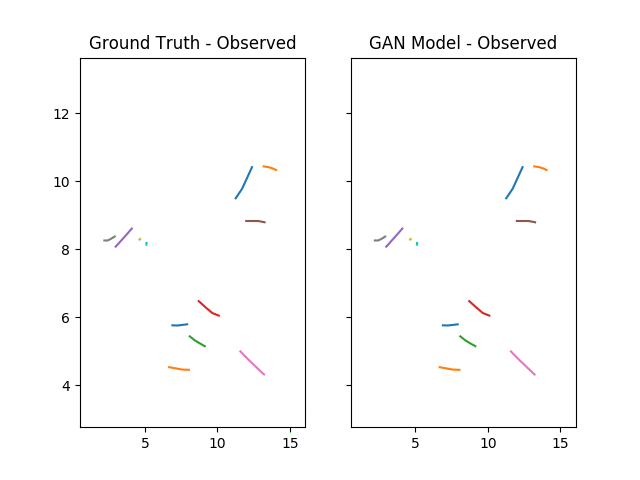
\includegraphics[width=\textwidth]{pictures/frames/chaotic_2/frame_03.png}
\caption[]
{{\small }}
\label{fig:chaotic2_1}
\end{subfigure}
\hfill
\begin{subfigure}[b]{0.475\textwidth}
\centering
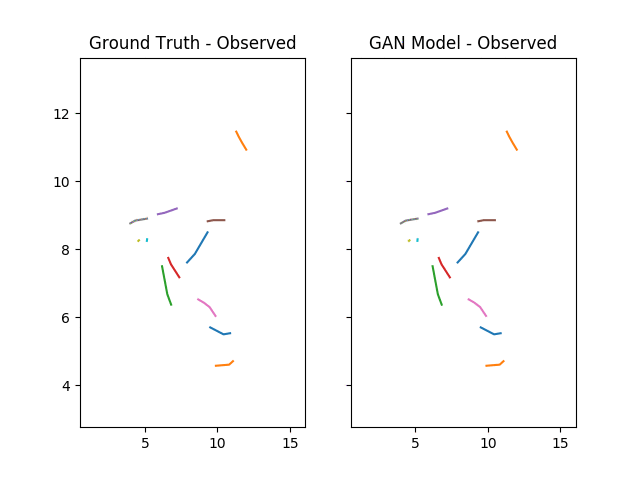
\includegraphics[width=\textwidth]{pictures/frames/chaotic_2/frame_10.png}
\caption[]
{{\small }}
\label{fig:chaotic2_2}
\end{subfigure}
\hfill
\vskip\baselineskip
\begin{subfigure}[b]{0.475\textwidth}
\centering
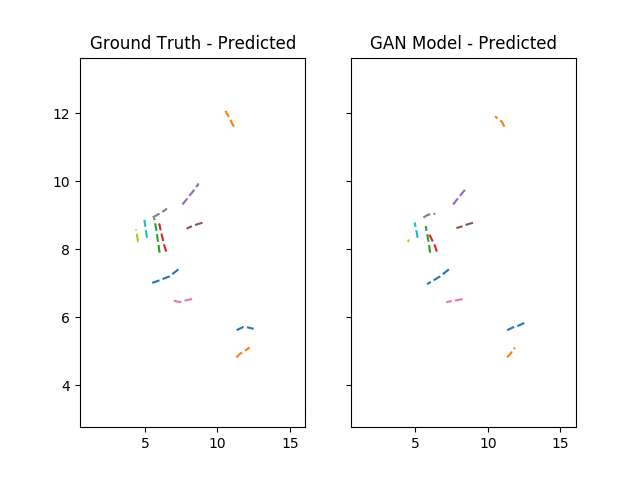
\includegraphics[width=\textwidth]{pictures/frames/chaotic_2/frame_14.png}
\caption[]
{{\small }}
\label{fig:chaotic2_3}
\end{subfigure}
\quad
\begin{subfigure}[b]{0.475\textwidth}
\centering
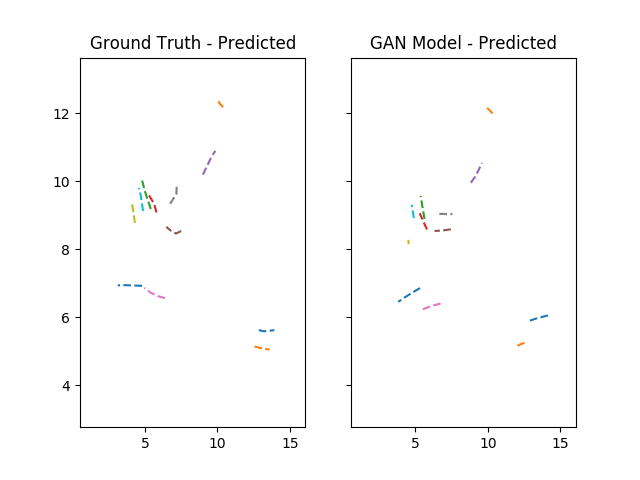
\includegraphics[width=\textwidth]{pictures/frames/chaotic_2/frame_18.png}
\caption[]
{{\small }}
\label{fig:chaotic2_4}
\end{subfigure}
\caption{Some observed and predicted frames of a bunch of pedestrians. The left graphs are the always the ground truth and the right graphs are the model's observed or predicted trajectories as seen in its title. The chronological order is \ref{fig:chaotic2_1}, \ref{fig:chaotic2_2}, \ref{fig:chaotic2_3}, \ref{fig:chaotic2_4}. The model manages to predict the trajectories such that the pedestrians avoid clashes and group members follow each other.}
\label{fig:chaotic2}
\end{figure}


\end{itemize}
\end{task}

\newpage
\bibliographystyle{plain}
\bibliography{literature}

\end{document}